%%%%%%%%%%%%%%%%%%%%%%%%%%%%%%%%%%%%%%%%%
% University Assignment Title Page
% LaTeX Template
% Version 1.0 (27/12/12)
%
% This template has been downloaded from:
% http://www.LaTeXTemplates.com
%
% Original author:
% WikiBooks (http://en.wikibooks.org/wiki/LaTeX/Title_Creation)
%
% License:
% CC BY-NC-SA 3.0 (http://creativecommons.org/licenses/by-nc-sa/3.0/)
%
% Instructions for using this template:
% This title page is capable of being compiled as is. This is not useful for
% including it in another document. To do this, you have two options:
%
% 1) Copy/paste everything between \begin{document} and \end{document}
% starting at \begin{titlepage} and paste this into another LaTeX file where you
% want your title page.
% OR
% 2) Remove everything outside the \begin{titlepage} and \end{titlepage} and
% move this file to the same directory as the LaTeX file you wish to add it to.
% Then add \input{./title_page_1.tex} to your LaTeX file where you want your
% title page.
%
%%%%%%%%%%%%%%%%%%%%%%%%%%%%%%%%%%%%%%%%%
%\title{Title page with logo}
%----------------------------------------------------------------------------------------
%	PACKAGES AND OTHER DOCUMENT CONFIGURATIONS
%----------------------------------------------------------------------------------------

\documentclass[12pt]{article}
\usepackage[ngerman]{babel}
\usepackage[utf8x]{inputenc}
\usepackage{amsmath}
\usepackage{nccmath}%for tiny matrices
\usepackage{graphicx}
\usepackage{grffile}%For .s in graphics
\usepackage[ngerman]{cleveref}%Für bessere References
\usepackage[colorinlistoftodos]{todonotes}
\usepackage{subcaption}%Für subfigures

\setlength\parindent{0pt} %Noindent for the whole document

\begin{document}

\begin{titlepage}

\newcommand{\HRule}{\rule{\linewidth}{0.5mm}} % Defines a new command for the horizontal lines, change thickness here

\center % Center everything on the page

%----------------------------------------------------------------------------------------
%	HEADING SECTIONS
%----------------------------------------------------------------------------------------

\textsc{\LARGE Georg-August-Universität Göttingen}\\[1.5cm] % Name of your university/college
\textsc{\Large }\\[0.5cm] % Major heading such as course name
\textsc{\large Numerische Strömungsmechanik}\\[0.5cm] % Minor heading such as course title

%----------------------------------------------------------------------------------------
%	TITLE SECTION
%----------------------------------------------------------------------------------------

\HRule \\[0.4cm]
{ \Large \bfseries Simulation mit FTCS- und BTCS-Verfahren}\\[0.4cm] % Title of your document
\HRule \\[1.5cm]

%----------------------------------------------------------------------------------------
%	AUTHOR SECTION
%----------------------------------------------------------------------------------------

\begin{minipage}{0.4\textwidth}
\begin{flushleft} \large
\emph{Author:}\\
Philip \textsc{Marszal} % Your name
\end{flushleft}
\end{minipage}
~
\begin{minipage}{0.4\textwidth}
\begin{flushright} \large
\emph{Prüfer:} \\
Prof. Dr. Andreas \textsc{Tilgner} % Supervisor's Name
\end{flushright}
\end{minipage}\\[2cm]

% If you don't want a supervisor, uncomment the two lines below and remove the section above
%\Large \emph{Author:}\\
%John \textsc{Smith}\\[3cm] % Your name

%----------------------------------------------------------------------------------------
%	DATE SECTION
%----------------------------------------------------------------------------------------

{\large \today}\\[2cm] % Date, change the \today to a set date if you want to be precise

%----------------------------------------------------------------------------------------
%	LOGO SECTION
%----------------------------------------------------------------------------------------


\includegraphics{logo_1.jpg}\\[1cm] % Include a department/university logo - this will require the graphicx package

%----------------------------------------------------------------------------------------

\vfill % Fill the rest of the page with whitespace

\end{titlepage}


\begin{abstract}
Your abstract.
\end{abstract}

\section{Einleitung}

\section{Problemstellung}

\begin{align}
  \frac{\partial T(\boldsymbol x, t)}{\partial t} + \text{Pe}~ \boldsymbol{u}_0\cdot \nabla T(\boldsymbol x, t) = \nabla^2 T(\boldsymbol x, t). \label{Gl:PDGL}
\end{align}

\section{Methoden}
Zur Simulation von Strömungsmechanikproblemen kommen eine Vielzahl verschiedener Verfahren in Frage.
Ein konzeptionell simples Verfahren, das häufig Anwendung findet, ist die \emph{Finite-Differenzen-Methode}.
Diese wird zum Lösen des hier gestellten Problems verwendet.
Andere Verfahren die zur Lösung dieser Art von Problem eingesetzt werden können sind \emph{Finite-Volumen-Methoden}, \emph{Finite-Elemente-Verfahren} und \emph{spektrale Verfahren}.
Bei fast allen Verfahren liegt die Diskretisierung des integrierten Systems durch ein Gitter zu Grunde, welches die theoretisch kontinuierliche Lösungsfunktion approximiert.
\subsection{Finite-Differenzen-Verfahren}
Um eine partielle Differentialgleichung numerisch zu integrieren, müssen die Ableitungen ersetzt werden durch diskret berechenbare Terme.
Ein naiver Ansatz ist die Näherung der Ableitung $T'(x)$ einer Funktion an einem Punkt durch den Differenzenquotienten.
\begin{align}
  T'(x) = \lim_{h\rightarrow 0}\frac{T(x+h)-T(x)}{h}.\label{Gl:dq1O}
\end{align}
Bei der Verwendung eines Gitters entspricht hier $h$ dem Abstand der zwei benachbarten Gitterpunkte.
Der Differenzenquotient in \cref{Gl:dq1O} entspricht dem Vorwärtsdifferenzenquotienten erster Ordnung in $h$.

Eine Approximation höherer Ordnung erhält man z.B. durch den zentralen Differenzenquotienten
\begin{align}
  T'(x) = \frac{T(x+h)-T(x-h)}{2h} + O(h^2),\label{Gl:dq2O}
\end{align}
oder für die zweite Ableitung als Vorwärtsdifferenzenquotient von $T'(x)$:
\begin{align}
  T''(x) = \frac{T(x+h)-2T(x)+T(x-h)}{h^2}+O(h^2).\label{Gl:dq2O2Abl}
\end{align}
Durch Kombinationen unterschiedlicher Differenzenquotienten können Näherungen höherer Ordnung erhalten werden.
\subsection{FTCS-Variante}
Verwendet man zur Diskretisierung der PDGL eine Vorwärtsdifferenz für die Zeitableitung und eine zentrale Differenz für die Ortsableitungen, so spricht man von einem \emph{FTCS}-Verfahren (\textbf{F}orwards \textbf{T}ime \textbf{C}entral \textbf{S}pace).
Diskretisiert man \cref{Gl:PDGL} auf diese Weise so erhält man die Differenzengleichung:
\begin{align}
  \begin{split}
  \frac{T^{n+1}_{i,j}-T^{n}_{i,j}}{\Delta t} + \text{Pe}~ u_{i,j} \frac{T^{n}_{i+1,j}-T^{n}_{i-1,j}}{\Delta x} + \text{Pe}~ v_{i,j} \frac{T^{n}_{i,j+1}-T^{n}_{i,j-1}}{\Delta y}\\
   =  \frac{T^{n}_{i+1,j}-2T^{n}_{i,j}+T^{n}_{i-1,j}}{\Delta x^2} +\frac{T^{n}_{i,j+1}-2T^{n}_{i,j}+T^{n}_{i,j-1}}{\Delta y^2}
 \end{split}\label{Gl:FTCS}
\end{align}
Diese Gleichung kann nun numerisch integriert werden, indem $T^{n+1}_{i,j}$ für jeden Gitterpunkt berechnet wird.
Allerdings ist darauf zu achten ob man $T^{n+1}_{i,j}$ am Rand berechnet, denn hier müssen die Randbedingungen in die Gleichung eingebaut werden.

Die Dirichlet Randbedingungen lassen sich unproblematisch für $T^{n}_{i,0}$ und $T^{n}_{i,N_y+1}$ einsetzen. Diese Gitterpunkte verändern sich nicht im Laufe der Zeit, müssen also nicht integriert werden.
Anders sieht dies allerdings für die Neumann Randbedingungen aus. Die Gitterpunkte mit $i=0$ und $i=N_x+1$ verändern sich sehr wohl im Laufe der Zeit.

Um zu vermeiden, dass man auf Gitterpunkte außerhalb des Gitters zugreift, muss man eine Vorwärtsdifferenz verwenden.
Eine Näherung zweiter Ordnung für die Ableitung $\frac{\partial T(\boldsymbol x,t)}{\partial x}$ bei $x=0$ und $x=1$ lässt sich mit \cref{Gl:forw2} berechnen:
\begin{align}
  \begin{split}
  T^{n+1}_{0,j} = -\frac{1}{3} \left( T^{n+1}_{2,j}-4T^{n+1}_{1,j}\right), \\
  T^{n+1}_{N_x+1,j} = -\frac{1}{3} \left( T^{n+1}_{N_x-1,j}-4T^{n+1}_{N_x,j}\right).
\end{split}\label{Gl:forw2}
\end{align}

Mit \cref{Gl:FTCS} und \cref{Gl:forw2} ist man nun in der Lage das das Problem zu simulieren.

\subsection{Die BTCS-Variante}
Im Gegensatz zu dem FTCS-Verfahren, welches ein explizites Verfahren zu Lösung von partiellen Differentialgleichungen darstellt, handelt es sich bei der \emph{BTCS}-Methode (\textbf{B}ackwards \textbf{T}ime \textbf{C}entral \textbf{S}pace) um ein implizites Verfahren.
Implizite Verfahren erfordern die Lösung eines Gleichungssystems ehe ein Zeitschritt durchgeführt werden kann.

Im BTCS-Verfahren wird die Zeitableitung durch eine Rückwärtsdifferenz diskretisiert. Dadurch entsteht in dem vorliegenden Problem zunächst ein lineares Gleichungssystem aus $(N_x+1)\cdot (N_y+1)$ Gleichungen für die $T^n_{i,j}$.
\begin{align}
  \begin{split}
  \frac{T^{n}_{i,j}-T^{n-1}_{i,j}}{\Delta t} + \text{Pe}~ u_{i,j} \frac{T^{n}_{i+1,j}-T^{n}_{i-1,j}}{\Delta x} + \text{Pe}~ v_{i,j} \frac{T^{n}_{i,j+1}-T^{n}_{i,j-1}}{\Delta y}\\
   =  \frac{T^{n}_{i+1,j}-2T^{n}_{i,j}+T^{n}_{i-1,j}}{\Delta x^2} +\frac{T^{n}_{i,j+1}-2T^{n}_{i,j}+T^{n}_{i,j-1}}{\Delta y^2}
 \end{split}\label{Gl:BTCS}
\end{align}
Führt man die Dirichlet-Randbedingungen ein so reduziert sich das Gleichungssystem auf $N_x \cdot (N_y-1)$ Gleichungen. Um die Neumann-Randbedingungen mit dem Gleichungssystem zu vereinigen betrachtet man den zentralen Differenzenquotienten an $x=0$ und $x=1$:
\begin{align}
  \left. \frac{\partial T}{\partial x}\right|_{x=0} = \frac{T^{n}_{1,j}-T^{n}_{-1,j}}{\Delta x} = 0, \nonumber
\end{align}
und einem analogen Quotienten für $x=1$. Mithilfe dieser Gleichungen lassen sich die Terme $T^{n}_{-1,j}$ und $T^{n}_{N_x+2,j}$ aus dem Gleichungssystem eliminieren und somit die Neumann-Randbedingungen in die Gleichungen einbauen.

Um dieses System zu lösen bietet es sich an das Gitter $T^n_{i,j}$ als $N_x \cdot (N_y-1)$ dimensionalen Vektor umzuschreiben.
Die Lösung des Systems entspricht dann einer Invertierung der Matrix $M$, die sich aus den Gleichungen als \cref{Gl:Matrix} ergibt.

\begin{align}
M=\left(\begin{medsize}\begin{smallmatrix}
(1.+4D)      & (v_{0,1}A-D) & 0          & ...       & -2D       & 0        &...       &&...       &&0    \\
-(v_{0,2}A+D) & (1.+4D)      & (v_{0,2}A-D) & 0         & ...      & -2D       &0       &&...       &&0    \\
0          &-(v_{0,3}A+D)  & (1.+4D)      &(v_{0,3}A-D) &0         &...       &       & &...       &&0 \\
...          & ...        &...         &...        &...       &...       &...       &...&...       &&0\\
...          &  ...       &-(u_{i,j}A+D)  &...        &-(v_{i,j}A+D)&(1.+4D)     &(v_{i,j}A-D)& ...      & (u_{i,j}A-D)&... 0\\
    ...         & ...        &...         &...        &...       &...       &...       &...&...       &&0\\
0          &...         &            &...        &           &         &-2D          &...       &-(v_{N_x+1,N_y}A+D) &(1.+4D)
\end{smallmatrix}\end{medsize}\right)\label{Gl:Matrix}
\end{align}



Hierbei wurde der Vektor $\boldsymbol T^n$ so gewählt, dass die Spalten des Gitters aneinander gehängt werden, sprich die Komponenten des Vektors laufen zunächst im $j$-Index durch : $\boldsymbol T^n = \left( T^n_{0,1}, T^n_{0,2}, ..., T^n_{0,N_y}, T^n_{1,1},...,T^n_{N_x+1,N_y} \right)$.
Die Terme $A=\frac{Pe~\Delta t}{\Delta x}$ und $D=\frac{\Delta t}{\Delta x^2}$ enstprechen den konstanten Vorfaktoren im Advektions- und Diffusionsterm.

\subsection{Der SOR-Algorithmus}
Die Matrix $M$ hat für vernünftige Gittergrößen und Zeitschritte $\Delta t$ die Eigenschaft, dass sie diagonal dominant ist. Also die Summe der Beträge der nicht-diagonalen Einträge in jeder Spalte nicht den Betrag des diagonalen Eintrags dieser Spalte übersteigt.

Für Matrizen mit dieser Eigenschaft liefert das sogenannte Gauß-Seidel-Verfahren eine approximative Lösung des Gleichungssystems $ M\boldsymbol x = \boldsymbol b$, die garantiert gegen die tatsächliche Lösung konvergiert.
Zunächst wird $M$ in eine Summe aus untere und oberer Dreiecksmatrix, $L$ und $U$, und der Diagonale $D$ zerlegt. Die Iterationsvorschrift des Gauß-Seidel-Verfahrens sieht nun wie folgt aus:
\begin{align}
  \boldsymbol x_{n+1} = (L+D)^{-1}(\boldsymbol b - U\boldsymbol x_{n}) \label{eq:gss}
\end{align}
Der Vorteil dieser Methode liegt darin, dass das Produkt von $(L+D)^{-1}$ mit einem Vektor einfach über Vorwärtssubstitution berechnet werden kann, dank der Dreiecksform von $L+D$.

Eine Weiterentwicklung des Gauß-Seidel-Algorithmus ist die \emph{successive overrelaxation}-Methode (SOR). Dazu wird \cref{eq:gss} zunächst durch den Korrekturvektor $\boldsymbol r_n = M\boldsymbol x_n -\boldsymbol b$ ausgedrückt.
Über den Relaxationsparameter $\omega$ kann nun die Konvergenz des Gauß-Seidel-Verfahrens erheblich beschleunigt werden.
Die Iterationsvorschrift des SOR-Algorithmus lautet:
\begin{align}
  \boldsymbol x_{n+1} = \boldsymbol x_n - \omega (L+D)^{-1}(\boldsymbol r_n) \label{eq:sor}
\end{align}
Für die Wärmetransportgleichung liegt der optimale Relaxationsparameter zwischen 0 und 2.


\section{Programmstruktur}
Zur Bearbeitung des Problems wurden die beiden Methoden, FTCS und BTCS, in zwei getrennten Programmen implementiert. Als interface mit den Programmen wurde eine Konfigurationsdatei erstellt, die es erlaubt Parameter der Algorithmen zu ändern, ohne das Programm neu komplilieren zu müssen.
Die Interaktion mit der Konfigurationsdatei wurde in der Headerdatei \emph{interface.h} implementiert, welche zudem sämtliche Funktionen zur Ausgabe der Ergebnisse beinhaltet.

Die Kernfunktionen der Integration befinden sich in der \emph{integration.h}-Datei. Diese sind die Initialisierungen der Temperaturfelder, des Quellfeldes und der Geschwindigkeitsfelder.
Außerdem sind einzelne Zeitschritte in den Funktionen \emph{FTCS()} und \emph{FTCS\_with\_Q()} zusammengefasst. Diese nehmen als Input das Temperaturfeld (call-by-reference), die Geschwindigkeitsfelder und das Quellfeld (call-by-value).
Die Entscheidung, welche Gleichung integriert werden soll, wird in der Konfigurationsdatei getroffen.


Die BTCS-Methode benötigt weitere Funktionen, die von dem betrachteten Problem abhängen. Dies sind Funktionen zum transformieren des Feldes in einen Vektor und zurück (\emph{reshape\_vector()} und \emph{shape\_back()}), die Einführung der Dirichlet-Randbedingungen in den Vektor (\emph{impose\_dirichlet()}) und die Initialisierung der Matrix $M$ (\emph{BCTS\_implicit\_Matrix()}).

Im BTCS Programm werden zudem algebraische Operationen benötigt, die in der Datei \emph{operations.h} definiert sind.
Dabei handelt es sich um standard Vektor-Matrix Operationen, aber auch die Triangularisierung der $M$-Matrix (\emph{triangularize()}) und das von der Problemstellung unabhängige SOR-Verfahren (\emph{SOR()}).

Innerhalb der Schleife über die Zeit wurde zudem eine Abfrage eingeführt, die zu in der Konfigurationsdatei definierten Zeitpunkten das aktuelle Temperaturfeld ausgibt.

Die Darstellung der Ergebnisse wurde mittels \emph{Python-Matplotlib} durchgeführt.


\begin{figure}\centering
  %\input{FTCSflow.pdf_tex}
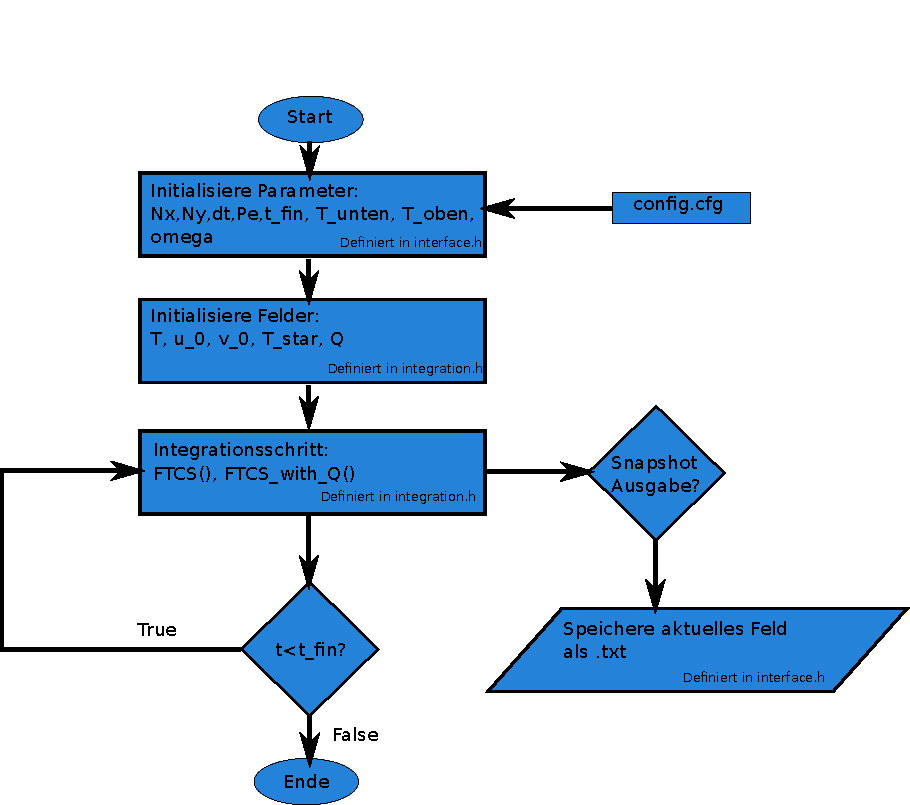
\includegraphics[width=0.4\textheight]{FTCSflow.pdf}\caption{Flowchart der Implementierung der FTCS-Methode.}\label{fig:FTCS}
\end{figure}

\begin{figure}\centering
  %\input{FTCSflow.pdf_tex}
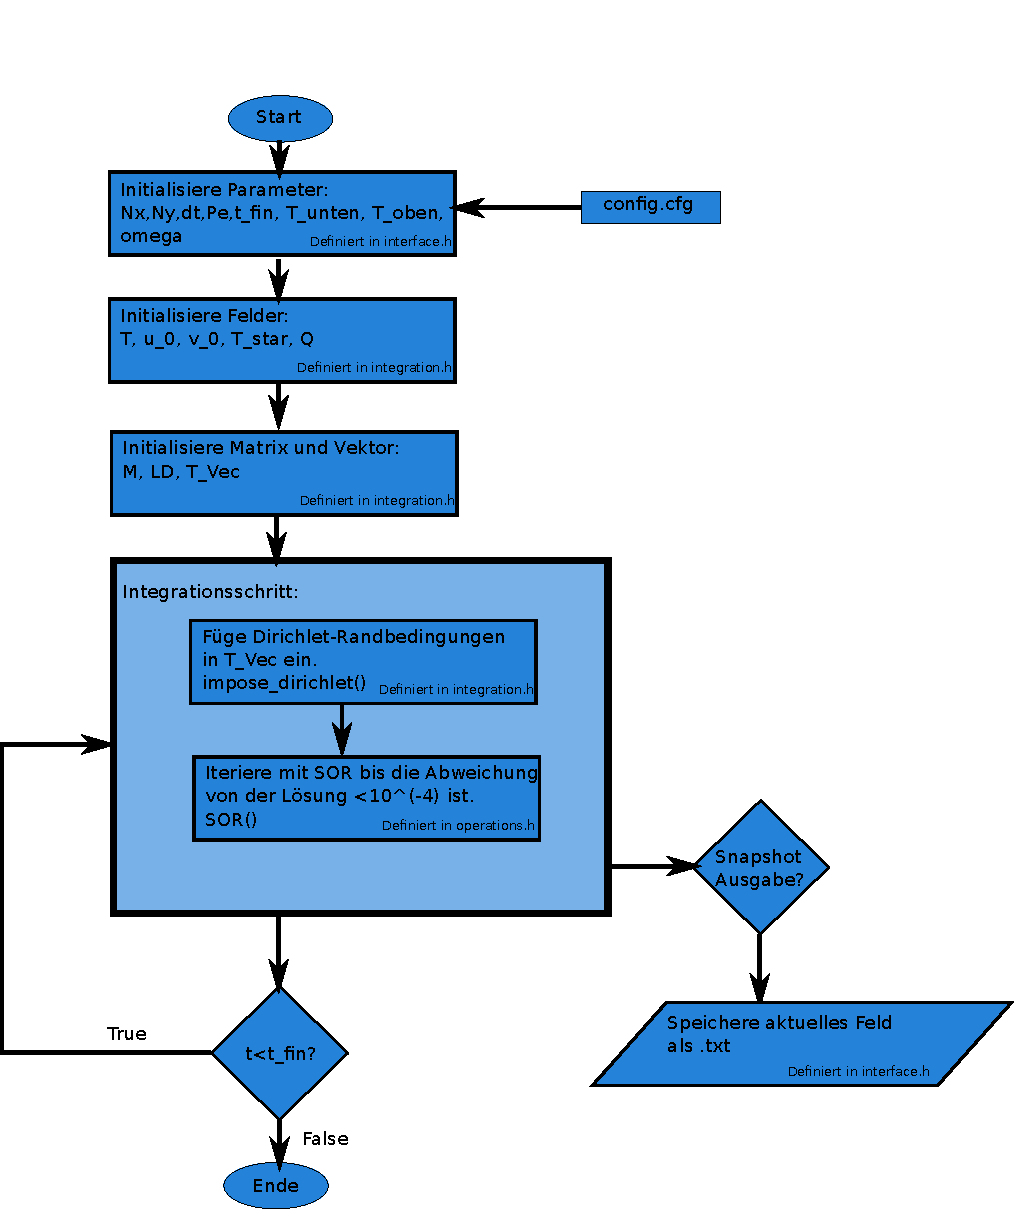
\includegraphics[width=0.4\textheight]{BTCSflow.pdf}\caption{Flowchart der Implementierung der BTCS-Methode.}\label{fig:BTCS}
\end{figure}

\section{Ergebnisse}
Die anfängliche Betrachtung des Temperaturfeldes im Verlauf der Zeit, wie es durch die FTCS-Methode berechnet wird, liefert die Ergebnisse in \cref{fig:FTCSnaive}. Hiefür wurde eine Peclet-Zahl von $Pe~=10$ und ein Gitter von $N_x=N_y=30$ angenommen. Die Schrittweite in der Zeit beträgt $dt=0.0002$.

\begin{figure}
\centering
  \begin{subfigure}[b]{0.48\textwidth}
    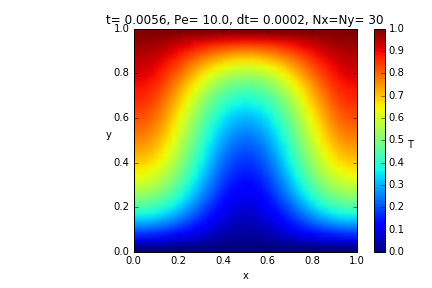
\includegraphics[width=1.15\textwidth]{/home/marszal/Projects/Num_Str_final/FTCS/plots/all/0.0056_10_30_30_0.0002_0.txt.png}
  \end{subfigure}
  ~
  \begin{subfigure}[b]{0.48\textwidth}
    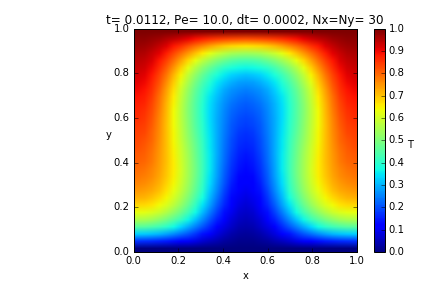
\includegraphics[width=1.15\textwidth]{/home/marszal/Projects/Num_Str_final/FTCS/plots/all/0.0112_10_30_30_0.0002_0.txt.png}
  \end{subfigure}
  \\
  \begin{subfigure}[b]{0.48\textwidth}
    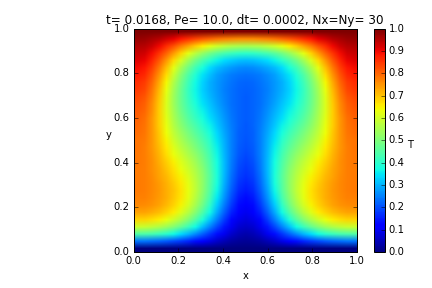
\includegraphics[width=1.15\textwidth]{/home/marszal/Projects/Num_Str_final/FTCS/plots/all/0.0168_10_30_30_0.0002_0.txt.png}
  \end{subfigure}
  ~
  \begin{subfigure}[b]{0.48\textwidth}
    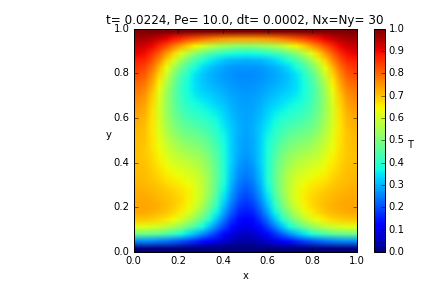
\includegraphics[width=1.15\textwidth]{/home/marszal/Projects/Num_Str_final/FTCS/plots/all/0.0224_10_30_30_0.0002_0.txt.png}
  \end{subfigure}
  \\
  \begin{subfigure}[b]{0.48\textwidth}
    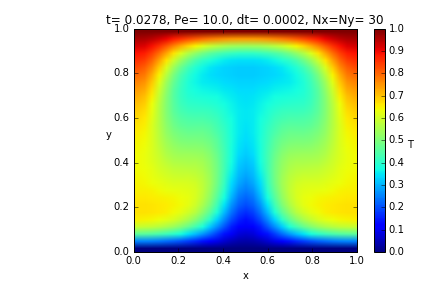
\includegraphics[width=1.15\textwidth]{/home/marszal/Projects/Num_Str_final/FTCS/plots/all/0.0278_10_30_30_0.0002_0.txt.png}
  \end{subfigure}
  ~
  \begin{subfigure}[b]{0.48\textwidth}
    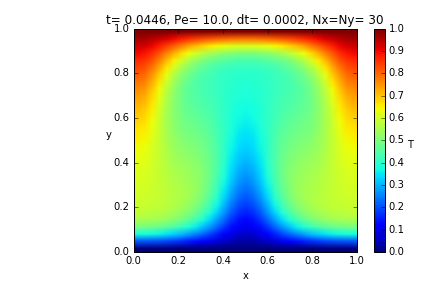
\includegraphics[width=1.15\textwidth]{/home/marszal/Projects/Num_Str_final/FTCS/plots/all/0.0446_10_30_30_0.0002_0.txt.png}
  \end{subfigure}
\caption{Temperaturfeld zu verschiedenen Zeiten. Berechnet mit dem FTCS-Verfahren.}\label{fig:FTCSnaive}
\end{figure}

Allerdings muss noch überprüft werden, wie genau das Ergebnis ist, und, wie die Gittergröße sich auf die Konvergenz auswirkt.

\section{Vergleich FTCS- und BTCS}

\end{document}
